\documentclass{beamer}
\usetheme{Madrid}
\usepackage{lmodern}
\usepackage{hyperref}
\usepackage{apacite}
\usepackage[utf8]{inputenc}
\usepackage[spanish]{babel}

\usepackage{xcolor}
\setbeamertemplate{background}{\tikz[overlay,remember picture]\node[opacity=0.2]at (current page.center){
\includegraphics[width=13cm]{KL.png}};}
\usepackage{tikz}
\usepackage{kantlipsum}

\setbeamercolor{normal text}{fg=black}

\begin{document}
\colorlet{beamer@blendedblue}{blue!46!green}
\setbeamercolor{normal text}{fg=black}

\setbeamercolor{frametitle}{fg=white, bg=blue!46!green}
\setbeamercolor*{title}{bg=blue!46!green, fg=white}

\setbeamercolor{section in toc}{fg=black}

\author[Juan C. Correa \textcolor{white}{(\url{https://correajc.com}})]{Juan C. Correa, Ph.D.}
\title[Enseñanza de la Transparencia Científica]{Entendiendo la Transparencia Científica y su Enseñanza}
% \subtitle{TREME}
	%\subtitle{}
\institute[]{Fundación Universitaria Konrad Lorenz\\
	\color{blue}\Email  \href{mailto:juanc.correan@konradlorenz.edu.co}{juanc.correan@konradlorenz.edu.co}}
\pgfdeclareimage[height=0.5cm]{KL}{KL}
\logo{\pgfuseimage{KL}}
\setbeamertemplate{caption}[numbered]
\date[Bogotá, Mayo-2021]{Curso en: \textbf{T}ecnologías \textbf{R}eproducibles en la \textbf{E}nseñanza de la \textbf{M}etodología y la \textbf{E}stadística}

%\subject{}
\setbeamercolor{background canvas}{bg=white}
%\setbeamertemplate{navigation symbols}{}

\begin{frame}
	\titlepage
\end{frame}

\begin{frame}
\begin{block}{Objetivo del Curso}
\vspace{0.3cm}
Comprender el concepto de Transparencia Científica y cómo puede enseñarse en cursos de metodología y estadística en psicología y otras ciencias sociales.  
\end{block}
\end{frame}



\begin{frame}
\frametitle{Agenda} 
\tableofcontents
\end{frame}

\section{Entendiendo la Transparencia Científica}
\begin{frame}{Entendiendo la Transparencia Científica}
Por \textcolor{blue!46!green}{Transparencia Científica} puede entenderse al conjunto de prácticas seguidas para maximizar la total comprensión de los procesos seguidos para el estudio de un fenómeno y divulgar este conocimiento en un artículo publicado en una revista científica.
\end{frame}



\begin{frame}{Entendiendo la Transparencia Científica}
Entendiendo las mejores prácticas de investigación en comparación con prácticas de investigación cuestionables \cite{Morling2020}.
\\
\vspace{0.5cm}
\begin{itemize}
    \item Prácticas cuestionables
    \begin{itemize}
        \item P-hacking
        \item Ocultar resultados 
        \item HARKing
    \end{itemize}
    \item Mejores Prácticas 
    \begin{itemize}
        \item Materiales Abiertos
        \item Datos Abiertos
        \item Pre-registro
        \item Reportar resultados de pre-registros
    \end{itemize}
\end{itemize}
\end{frame}

\begin{frame}{Entendiendo la Transparencia Científica}
\begin{figure}
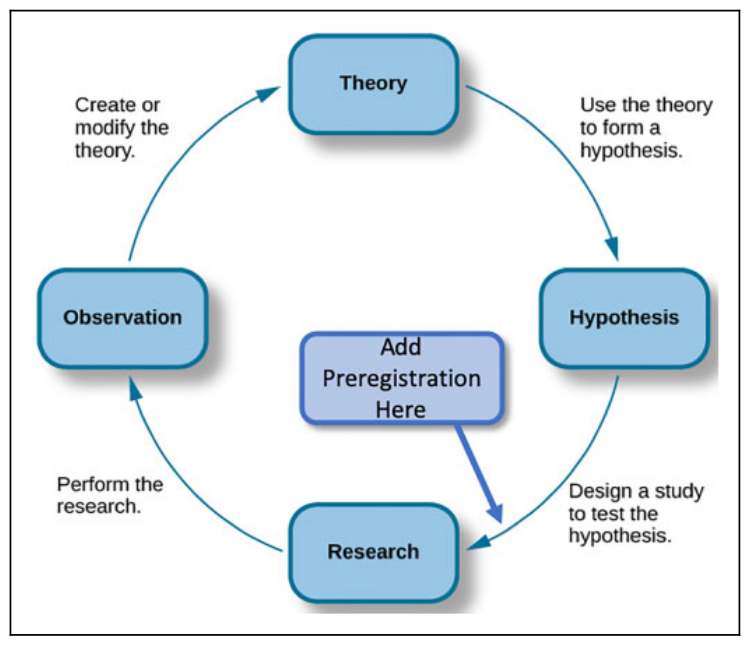
\includegraphics[width=.6\textwidth]{RC.png}
\end{figure}
\end{frame}


\section{Beneficios de la Transparencia Científica}
\begin{frame}{Beneficios de la Transparencia Científica}
Para Docentes:
\begin{itemize}
    \item Docencia de contenidos más actualizados
    \item Aprendizaje basado en la colaboración
    \item Aumento de oportunidades laborales
    \item Desarrollo profesional como investigador
\end{itemize}
Para Investigadores:
\begin{itemize}
    \item Aumento de citas (Mayor visibilización)
    \item Aumento en la conexión con otros colaboradores
    \item Aumento en la obtención de financiamientos
\end{itemize}
\end{frame}

\begin{frame}{Beneficios de la Transparencia Científica}
\begin{figure}
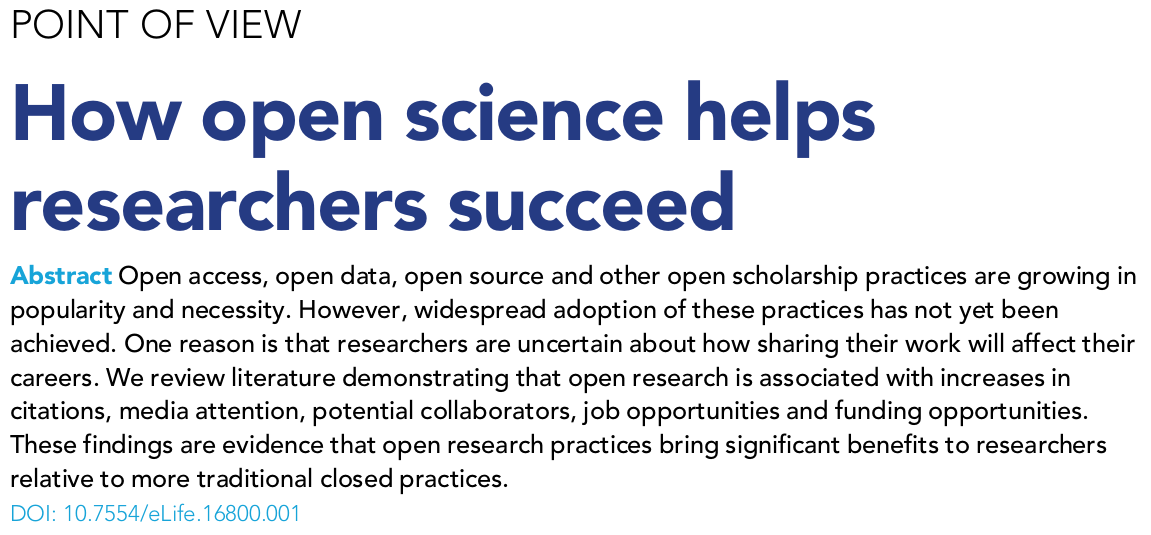
\includegraphics[width=1\textwidth]{OSB.png}
\end{figure}
\cite{Mckiernan2016}
\end{frame}

\section{Introducción a las Tecnologías Reproducibles}
\begin{frame}{Introducción a las Tecnologías Reproducibles}
Por \textcolor{blue!46!green}{Tecnologías Reproducibles} se entiende al conjunto de herramientas tecnológicas (fundamentalmente de software) que están disponibles para seguir prácticas de Transparencia Científica \cite{Mair2016}.
\begin{figure}
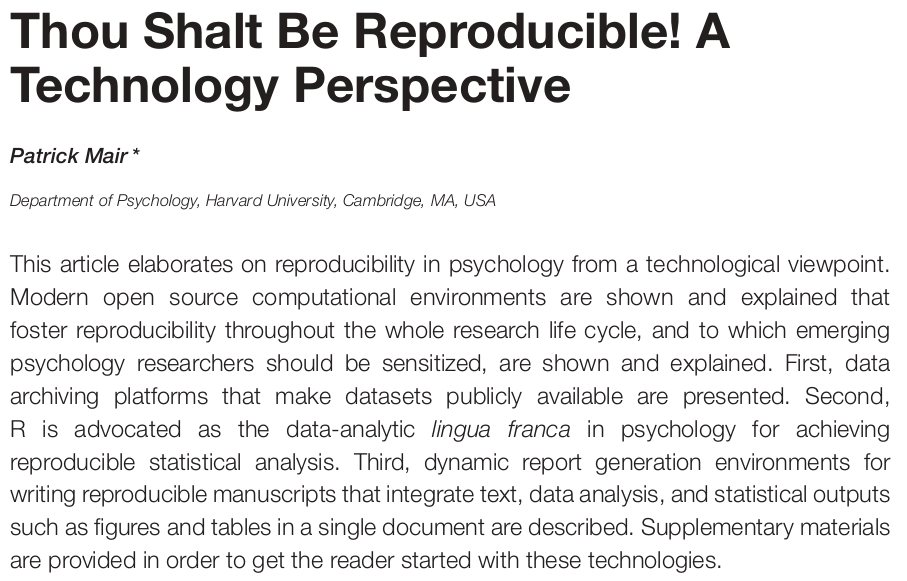
\includegraphics[width=.5\textwidth]{TR.png}
\end{figure}
\end{frame}

\begin{frame}{Introducción a las Tecnologías Reproducibles}
\begin{figure}
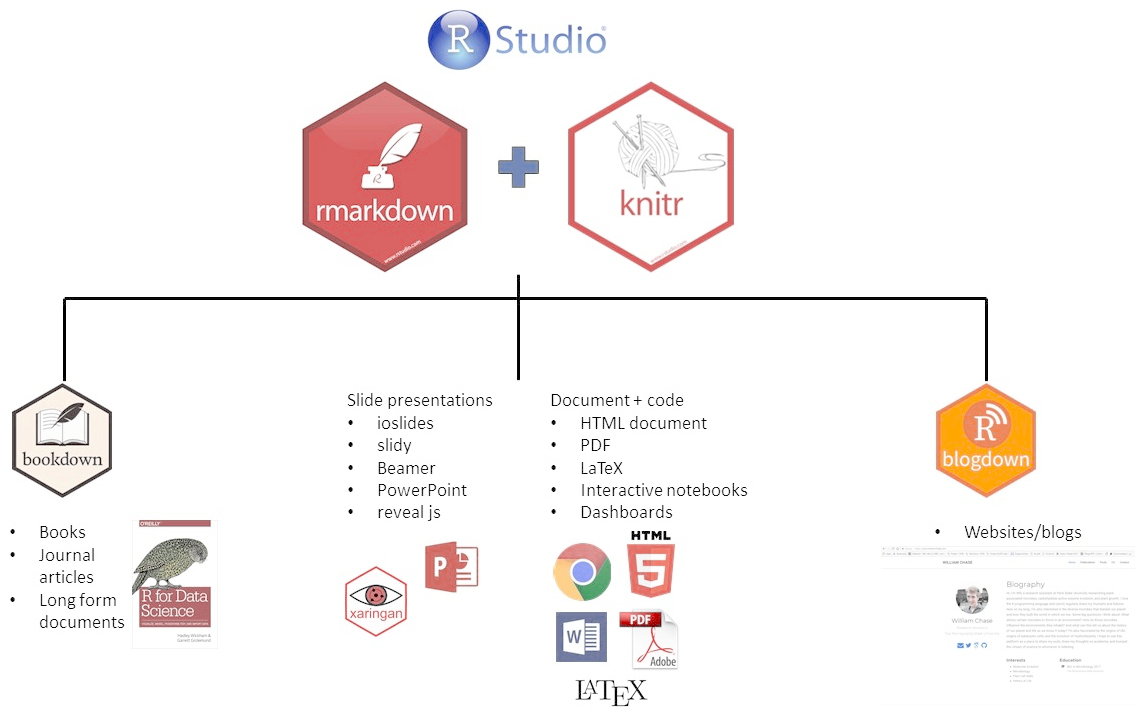
\includegraphics[width=.8\textwidth]{tools.png}
\end{figure}
\end{frame}

\begin{frame}{Introducción a las Tecnologías Reproducibles}
\begin{figure}

\includegraphics[width=1\textwidth]{Preprints.png}
\end{figure}
\end{frame}

\begin{frame}{Introducción a las Tecnologías Reproducibles}
Acá se tiene un ejemplo de un recurso en línea que promueve la enseñanza de la teoría de respuesta al ítem a través de un artículo disponible en PsyArXiv Preprints.
\begin{figure}
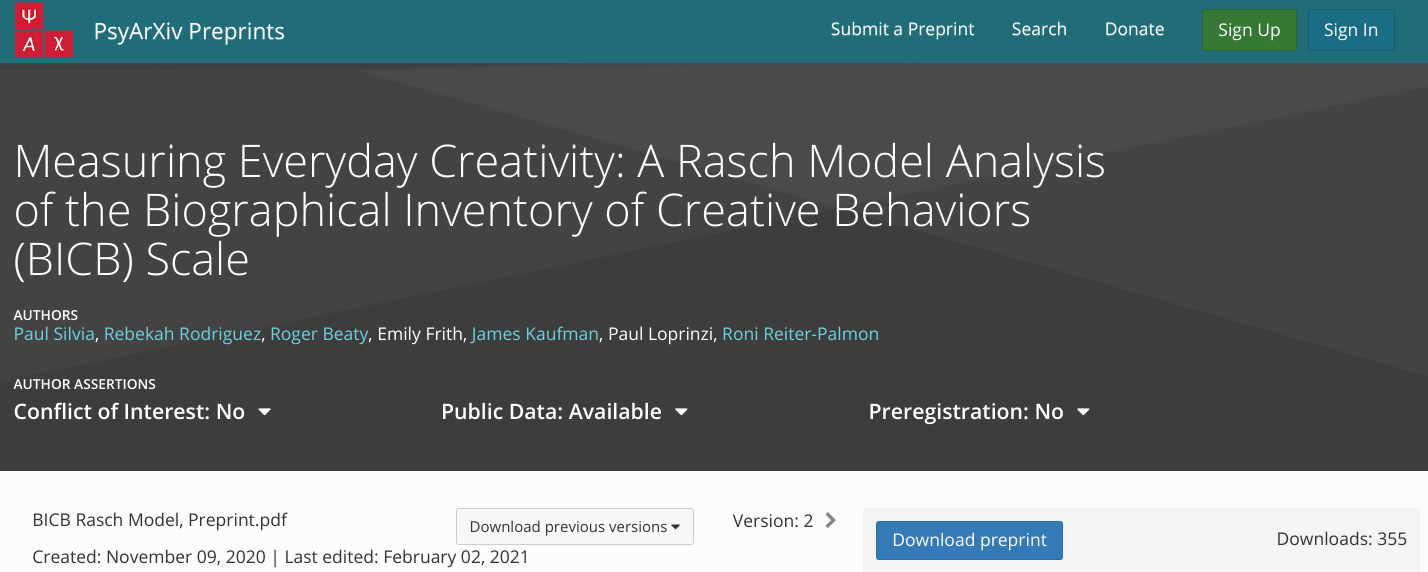
\includegraphics[width=1\textwidth]{Ejemplo.png}
\end{figure}
\textcolor{blue}{\url{https://psyarxiv.com/3wq7c/}}
\end{frame}

\begin{frame}[allowframebreaks]{Referencias}
\tiny
\bibliographystyle{apacite}
\bibliography{refs} 
\end{frame}


\end{document}